\let\negmedspace\undefined
\let\negthickspace\undefined
\documentclass[journal,12pt,twocolumn]{IEEEtran}
\usepackage{cite}
\usepackage{amsmath,amssymb,amsfonts,amsthm}
\usepackage{algorithmic}
\usepackage{graphicx}
\usepackage{textcomp}
\usepackage{xcolor}
\usepackage{txfonts}
\usepackage{listings}
\usepackage{enumitem}
\usepackage{mathtools}
\usepackage{gensymb}
\usepackage{comment}
\usepackage[breaklinks=true]{hyperref}
\usepackage{tkz-euclide}
\usepackage{listings}
\usepackage{gvv}
\def\inputGnumericTable{}
\usepackage[latin1]{inputenc}
\usepackage{color}
\usepackage{array}
\usepackage{longtable}
\usepackage{calc}
\usepackage{multirow}
\usepackage{hhline}
\usepackage{ifthen}
\usepackage{lscape}

\newtheorem{theorem}{Theorem}[section]
\newtheorem{problem}{Problem}
\newtheorem{proposition}{Proposition}[section]
\newtheorem{lemma}{Lemma}[section]
\newtheorem{corollary}[theorem]{Corollary}
\newtheorem{example}{Example}[section]
\newtheorem{definition}[problem]{Definition}
\newcommand{\BEQA}{\begin{eqnarray}}
\newcommand{\EEQA}{\end{eqnarray}}
\newcommand{\define}{\stackrel{\triangle}{=}}
\theoremstyle{remark}
\newtheorem{rem}{Remark}
\begin{document}

\bibliographystyle{IEEEtran}
\vspace{3cm}

\title{NCERT Discrete - 10.5.2.2}
\author{EE23BTECH11058 - Sindam Ananya$^{*}$% <-this % stops a space
}
\maketitle
\newpage
\bigskip

\renewcommand{\thefigure}{\theenumi}
\renewcommand{\thetable}{\theenumi}

\vspace{3cm}
\textbf{Question 10.5.2.2:} 
\begin{enumerate}
\item 30th term of the AP: 10, 7, 4, $\ldots$ is 
\item 11th term of the AP: $-3, -\frac{1}{2}, 2, \ldots$ is
\end{enumerate}
\solution
\begin{table}[h!]
    \centering
    \begin{tabular}{ | c | c | c | }
        \hline
        \textbf{Parameter}  & \textbf{value} & \textbf{Description} \\
        \hline
        \multirow{2}{*}{\begin{tabular}[c]{@{}c@{}}$x_i(0)$\\  \end{tabular}} & 10 & \multirow{2}{*}{\begin{tabular}[c]{@{}c@{}}First \\ term\end{tabular}} \\
        \cline{2-2}
        & -3 &  \\
        \hline
        \multirow{2}{*}{\begin{tabular}[c]{@{}c@{}}$d_i$ \\ \end{tabular}} & -3 & \multirow{2}{*}{\begin{tabular}[c]{@{}c@{}}Common \\ difference\end{tabular}} \\
        \cline{2-2}
          & $\frac{5}{2}$ &  \\
        \hline
        $x_1(29)$ &  ? & 30th term \\
        \hline
        $x_2(10)$ & ? & 11th term \\
        \hline
    \end{tabular}

    \caption{Input Parameters}
    \label{table:1}
    \end{table}\\
1)Let the AP be a function $x_1(n)$ where $x_1(n)$ is the $(n+1)th$ term of AP(1).\\
Let the common difference be $d_1$.\\
So, the first term is $x_1(1-1)$ which is $x_1(0)$; given $x_1(0) = 10$\\ 
For the 30th term of the series we need to find $x_1(30-1)$ which is $x_1(29)$.\\
Let Z-transform of $x_1(n)$ be $X_1(z)$. Let $U(z)$ be the Z-transform of $u(n)$.\\
where \(u(n)\) is the step function.
\begin{align}
x_1(n) &= [x_1(0) + (n) \times d_1 ]\times u(n)\\
X_1(z) &= x_1(0).U(z) + d_1(Z\{nu(n)\})\\
       &= \frac{x_1(0)}{1-z^{-1}} + \frac{d_1\times z^{-1}}{(1-z^{-1})^2}\\
       &= \frac{10}{1-z^{-1}} + \frac{(-3)z^{-1}}{(1-z^{-1})^2}\\
       &= \frac{10}{1-z^{-1}} - \frac{3z^{-1}}{(1-z^{-1})^2}\\
       &= \frac{10 - 13z^{-1}}{(1-z^{-1})^2} \quad \forall \quad |z| > 1
\end{align}
From the values given in table:1 :
\begin{align}
x_1(29) &= (10 + (29)(-3))(u(n))\\
&= (10 + 29(-3))(u(n))\\
&= (10+ (-87))(u(n))  \\
&= -77
\end{align}
(where $u(n) = 1$ if $n \geq 0$ )\\
                 
So, the 30th term of the AP is $-77$.\\
\begin{figure}[h!]
    \centering
    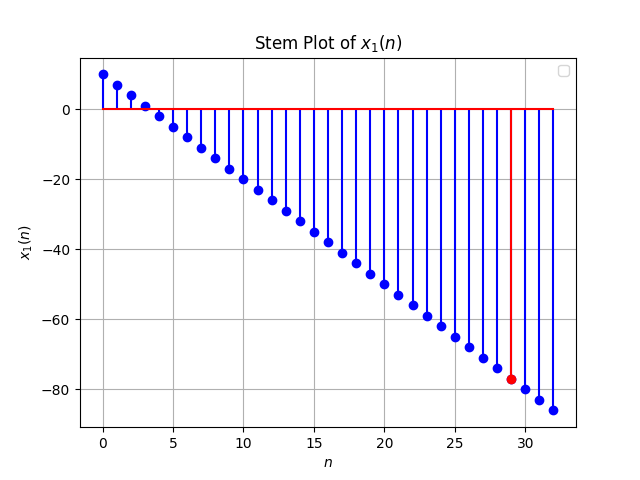
\includegraphics[width=\columnwidth]{figs/plot1.png}
    \label{fig:1}
\end{figure}

2)Let the AP be a function $x_2(n)$ where $x_2(n)$ is the $(n+1)th$ term of AP(2).\\
Let the common difference be $d_2$.\\
So, the first term is $x_2(1-1)$ which is $x_2(0)$; given $x_2(0) = -3$\\ 
For the 11th term of the series we need to find $x_2(11-1)$ which is $x_2(10)$.\\
Let Z-transform of $x_1(n)$ be $X_1(z)$. Let $U(z)$ be the Z-transform of $u(n)$.\\
where \(u(n)\) is the step function.
\begin{align}
x_2(n) &= [x_2(0) + (n) \times d_2 ]\times u(n)\\
X_2(z) &= x_2(0).U(z) + d_2(Z\{nu(n)\})\\
       &= \frac{x_2(0)}{1-z^{-1}} + \frac{d_2\times z^{-1}}{(1-z^{-1})^2}\\
       &= \frac{-3}{1-z^{-1}} + \frac{(2.5)z^{-1}}{(1-z^{-1})^2}\\
       &= \frac{0.5z^{-1}-3}{(1-z^{-1})^2} \quad \forall \quad |z| > 1
\end{align}
From the values given in table:1 :
\begin{align}
x_2(10) &= (-3 + (10)\left(\frac{5}{2}\right))(u(n))\\
&= (-3 + 10(2.5))(u(n))\\
& = (-3 + 25)(u(n)) \\
&= 22
\end{align}
(where $u(n) = 1$ if $n \geq 0$ )\\

\begin{figure}[h!]
    \centering
    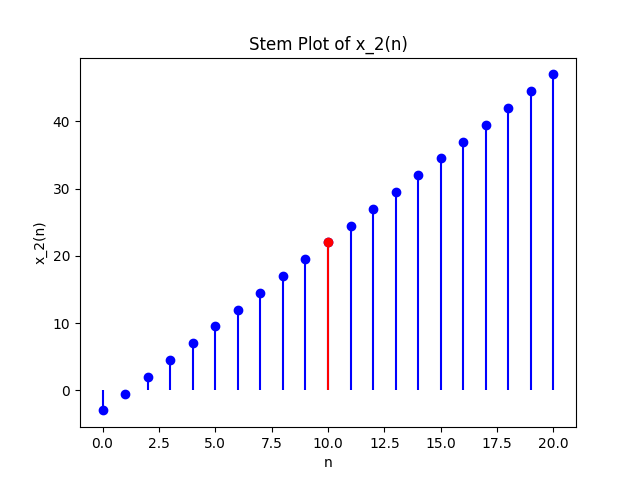
\includegraphics[width=\columnwidth]{figs/plot2.png}
    \label{fig:2}
\end{figure}
so, the 11th term of the AP is $22$.
\end{document}
